\section{Results}
\label{sec:results}

% AUTO-GENERATED by research_rescue/make_tables_v2.py from results/v2 - do not edit by hand.
\begin{table*}[t]
\centering
\caption{Real cars (LiRA-CD), leave-one-route-out, 100\,m segments. Within-route metrics and partial $\rho$ as defined in Section~\ref{sec:method}. $\Delta$MAE: paired difference to the real-trained LightGBM with a 95\,\% cluster-bootstrap interval over 5\,km blocks (40 clusters); ``routes'': number of held-out routes on which the estimator is better. Neural nets: 5-seed ensembles.}
\label{tab:real}
\setlength{\tabcolsep}{4pt}
\footnotesize
\begin{tabular}{@{}lcccccrc@{}}
\toprule
Estimator & \multicolumn{3}{c}{Within route} & \multicolumn{2}{c}{Pooled} & $\Delta$MAE vs M3 & Routes \\
\cmidrule(lr){2-4}\cmidrule(lr){5-6}
 & MAE & $\rho$ & partial $\rho$ & MAE & bias & [5\,km-block CI] & better \\
\midrule
\multicolumn{8}{@{}l}{\emph{No vibration input}} \\
\quad M0 constant (training median) & 1.56 & -- & -- & 1.67 & $-$0.64 & +1.249 [+1.118, +1.387] & 0/4 \\
\quad M0b road-class prior (map only) & 0.75 & -- & -- & 0.81 & $-$0.20 & +0.387 [+0.307, +0.475] & 0/4 \\
\quad M1 speed only & 0.69 & 0.39 & 0.19 & 0.74 & $-$0.33 & +0.324 [+0.252, +0.404] & 0/4 \\
\multicolumn{8}{@{}l}{\emph{Physics-based, calibrated on real training routes}} \\
\quad M2c vibration index & 0.62 & 0.76 & 0.77 & 0.67 & $-$0.13 & +0.251 [+0.202, +0.306] & 0/4 \\
\quad M7 quarter-car inversion & 0.46 & 0.82 & 0.81 & 0.49 & $-$0.08 & +0.074 [+0.039, +0.105] & 0/4 \\
\quad M7 + output calibration & 0.54 & 0.82 & 0.81 & 0.58 & +0.05 & +0.155 [+0.109, +0.201] & 0/4 \\
\multicolumn{8}{@{}l}{\emph{Learned on real cars (3 other routes)}} \\
\quad M3 LightGBM (reference) & 0.39 & 0.83 & 0.81 & 0.42 & $-$0.11 & ref. & -- \\
\quad M3 LightGBM, no speed input & 0.62 & 0.76 & 0.72 & 0.65 & $-$0.24 & +0.235 [+0.177, +0.294] & 0/4 \\
\quad M4 MLP & 0.40 & 0.83 & 0.81 & 0.42 & $-$0.09 & +0.004 [$-$0.013, +0.023] & 0/4 \\
\quad M5 1D-CNN & 0.43 & 0.81 & 0.79 & 0.47 & $-$0.21 & +0.045 [+0.019, +0.075] & 1/4 \\
\multicolumn{8}{@{}l}{\emph{Learned on simulation only (zero-shot)}} \\
\quad V0 LightGBM, measured profiles & 0.42 & 0.83 & 0.81 & 0.44 & +0.01 & +0.019 [$-$0.003, +0.040] & 1/4 \\
\quad V10 LightGBM, measured + synthetic & 0.44 & 0.84 & 0.82 & 0.46 & $-$0.04 & +0.039 [+0.007, +0.068] & 2/4 \\
\bottomrule
\end{tabular}
\end{table*}


\subsection{Real cars}
\label{sec:res_real}
Table~\ref{tab:real} lists every estimator on the held-out routes (per route: Table~\ref{S-tab:s_routes}).
A map alone (M0b) or speed alone (M1) gives within-route MAEs of \vrMapMaeWithin{} and \vrSpeedMaeWithin\,m/km.
The calibrated quarter-car inversion M7 ranks segments as well as the learned estimators ($\rho=$\,\vrInvRhoWithin) but has a larger error (paired difference to LightGBM \vrInvDfive{} [\vrInvDfiveLo, \vrInvDfiveHi]\,m/km), and its output calibration on the training routes made it worse.
LightGBM and the MLP differ negligibly (\vrMlpDfive{} [\vrMlpDfiveLo, \vrMlpDfiveHi]); the 1D-CNN of our earlier study is worse by \vrCnnDfive{} [\vrCnnDfiveLo, \vrCnnDfiveHi], almost entirely on CPH1.
LightGBM's MAE is \vrGbmMaeCphOne{} and \vrGbmMaeCphSix\,m/km on the urban routes and \vrGbmMaeMwThree{} and \vrGbmMaeMwThirteen\,m/km on the motorways, or \reGbmUrban\,\% and \reGbmMotorway\,\% of the mean IRI of each class (Table~\ref{S-tab:s_relerr}).
The same telematics units drive several routes, but LightGBM trained only on units that never drove the held-out route is as accurate as on size-matched random subsets (Table~\ref{S-tab:s_unit}; the M3 fold is not interpretable), so vehicle overlap did not measurably favour the real-trained estimators (the within-road split of Bajic et al.~\cite{bajic2021ml} is in Table~\ref{S-tab:s_bajic}).

\subsection{Zero-shot transfer: the ranking transfers, the level does not}
\label{sec:res_zero}
Trained only on simulated drives over the profiles of the three training routes, the pre-specified simulator V0 reaches a within-route MAE of \vrSimVzeroMaeWithin\,m/km against \vrGbmMaeWithin{} for the real-trained model.
The paired difference, \vrSimVzeroDfive\,m/km, has a 5\,km-block interval of [\vrSimVzeroDfiveLo, \vrSimVzeroDfiveHi], whereas a segment-level interval, which ignores spatial dependence, would have declared the real-trained model better (Table~\ref{S-tab:s_inference}).
Both rank segments within routes alike ($\rho=$\,\vrSimVzeroRhoWithin{} vs \vrGbmRhoWithin; partial $\rho$ given speed \vrSimVzeroPrhoWithin{} vs \vrGbmPrhoWithin).
Within-route ranking discriminates little, however, because a Spearman correlation within a route is unaffected by any monotone calibration: the untrained statistic RMS$/v^{0.5}$ reaches $\rho=$\,\rkHalfRho{} (partial \rkHalfPrho).
Paired on the same segments (Table~\ref{S-tab:s_rank}), real-trained LightGBM ranks the urban routes better than this statistic (by \rpRhoRealCphOne{} and \rpRhoRealCphSix) and the motorways slightly worse (\rpRhoRealMwThree{} and \rpRhoRealMwThirteen), and V0-trained LightGBM differs from it by \rpRhoVzeroMwThirteen{} to \rpRhoVzeroCphOne; real-, V0- and V1-trained LightGBM are within \rpAbsMax{} of it on every route, as are, in point estimates, the other variants, the MLP, the CNN and M7 (Table~\ref{S-tab:s_rank}).
What training has to supply is mainly the level of the mapping from vibration to IRI.

% AUTO-GENERATED by research_rescue/make_tables_v3.py from results/v2 and results/v3 - do not edit by hand.
\begin{table*}[t]
\centering
\caption{Simulator variants: LightGBM trained only on simulated drives (zero-shot), tested on the held-out real routes. Pooled segment MAE and bias in m/km; level: mean log(prediction/label) over the segments of a route, averaged over the two routes of a road class (0.10 is about 10\,\% over-prediction); within-route Spearman $\rho$. Right: pooled MAE with 5 or 20\,km of paired drives (about ten passes per segment) used for a level offset (2.5--97.5\,\% range over the 20 draws in brackets) or for joint training; means over 20 draws. Real-only LightGBM on the same drives: \vbRealOnlyFive\,m/km (5\,km), \vbRealOnlyTwenty\,m/km (20\,km). Class E except V0. Scale $b$ and speed elasticities: Table~\ref{S-tab:variants_s_gbm}.}
\label{tab:variants}
\setlength{\tabcolsep}{3.2pt}
\scriptsize
\begin{tabular}{@{}lcccccccccc@{}}
\toprule
& \multicolumn{5}{c}{Zero-shot} & \multicolumn{2}{c}{+ level offset} & \multicolumn{2}{c}{+ joint training} \\ \cmidrule(lr){2-6}\cmidrule(lr){7-8}\cmidrule(lr){9-10}
Simulator variant & MAE & bias & level urban & level motorway & $\rho$ & 5\,km & 20\,km & 5\,km & 20\,km \\
\midrule
V0 mixture (reference, pre-specified) & 0.44 & +0.01 & +0.01 & +0.14 & 0.83 & 0.42 [0.40, 0.45] & 0.42 & 0.45 & 0.44 \\
V1 telematics-like, rigid & 0.68 & +0.43 & +0.14 & +0.40 & 0.83 & 0.53 [0.47, 0.60] & 0.54 & 0.47 & 0.44 \\
V7 telematics-like + holder & 0.46 & +0.07 & +0.02 & +0.18 & 0.83 & 0.43 [0.40, 0.46] & 0.43 & 0.46 & 0.44 \\
V8 phone-like, rigid & 0.55 & +0.27 & +0.10 & +0.26 & 0.84 & 0.45 [0.42, 0.49] & 0.46 & 0.45 & 0.44 \\
V2 phone-like + holder & 0.41 & $-$0.09 & $-$0.03 & +0.06 & 0.83 & 0.42 [0.40, 0.45] & 0.41 & 0.45 & 0.43 \\
V3 ideal sensor & 0.67 & +0.40 & +0.13 & +0.40 & 0.83 & 0.54 [0.48, 0.62] & 0.55 & 0.47 & 0.45 \\
V5 telematics matched to LiRA-CD & 0.69 & +0.40 & +0.12 & +0.42 & 0.82 & 0.56 [0.51, 0.64] & 0.58 & 0.47 & 0.44 \\
V6 matched telematics + phone-like & 0.46 & $-$0.04 & $-$0.03 & +0.19 & 0.83 & 0.45 [0.41, 0.48] & 0.45 & 0.45 & 0.43 \\
V4 one mid-range vehicle & 0.63 & +0.40 & +0.16 & +0.29 & 0.83 & 0.44 [0.41, 0.46] & 0.43 & 0.47 & 0.44 \\
V10 measured + synthetic profiles & 0.46 & $-$0.04 & $-$0.04 & +0.20 & 0.84 & 0.46 [0.41, 0.50] & 0.46 & 0.45 & 0.43 \\
V9 synthetic profiles only & 0.71 & +0.36 & +0.07 & +0.49 & 0.81 & 0.75 [0.65, 0.88] & 0.77 & -- & -- \\
\midrule
trained on real cars (M3) & 0.42 & $-$0.11 & $-$0.01 & +0.02 & 0.83 & -- & -- & -- & -- \\
\bottomrule
\end{tabular}
\end{table*}


\begin{figure*}[t]
\centering
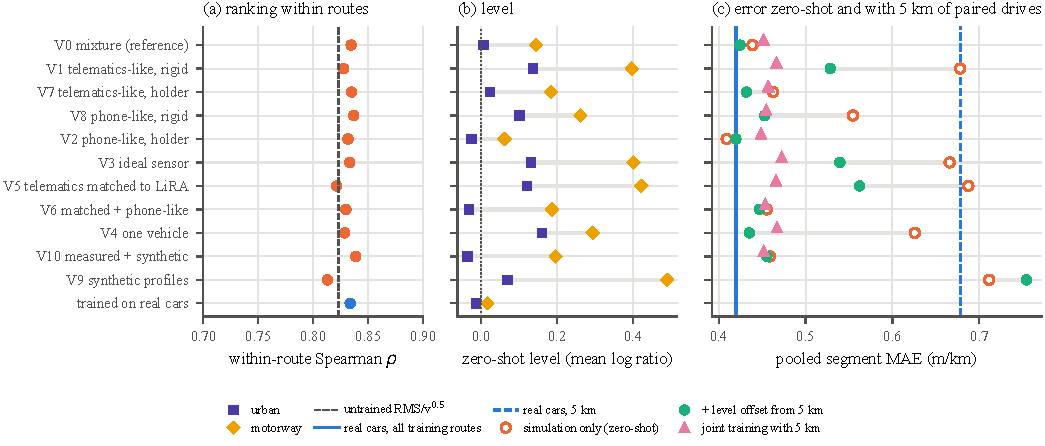
\includegraphics[width=\textwidth]{v3_variants.pdf}
\caption{Simulator variants, LightGBM trained on simulated drives only and tested on the held-out real routes. (a) Within-route Spearman $\rho$. (b) Zero-shot level (mean log ratio of prediction to label; mean of a class's two routes). (c) Pooled segment MAE zero-shot and with 5\,km of paired drives (means over 20 draws).}
\label{fig:variants}
\end{figure*}

V0's agreement in level is not a robust property of simulating over measured profiles (Table~\ref{tab:variants}, Fig.~\ref{fig:variants}).
Across the nine variants on measured profiles (V0--V8), the within-route $\rho$ stays between \vvRhoMin{} and \vvRhoMax{} and the scale $b$ between \vvScaleMin{} and \vvScaleMax{} (real-trained: \vvRealScaleB), whereas the pooled zero-shot bias ranges from \vvBiasMin{} to \vvBiasMax\,m/km.
Even V0 matches the level only on average: its pooled bias of \vrSimVzeroBias\,m/km combines a matched urban level (log level \ldVzeroUrban) with a motorway over-prediction of about \ldVzeroPctMotorwayAbs\,\% (\ldVzeroMotorway; real-trained \ldRealUrban{} and \ldRealMotorway).
In the 2$\times$2 sensor design, adding the holder resonance changes the bias by \vvHolderEffTele{} and \vvHolderEffPhone\,m/km for the telematics-like and the phone-like sensor, and switching the sensor family by \vvFamilyEffRigid{} and \vvFamilyEffHolder\,m/km without and with holder.
The vehicle population moves it as much: with V0's sensor mixture, holder resonance included, but one mid-range vehicle instead of 30 (V4), the bias rises by \vpVehicleEffBias\,m/km.
V0's level thus comes from both its holder resonance (meant for phone holders, not the car's telematics unit) and its 30-vehicle population.
An ideal sensor (V3) and a telematics sensor matched to the rates, quantisation, noise and tilt of the LiRA-CD streams (V5) both overestimate by about 0.4\,m/km.
Synthetic profiles alone (V9) still rank segments ($\rho=$\,\vvVnineRhoWithin) but overestimate on motorways, and the earlier game-engine corpus does not transfer ($\rho=$\,\vvBcorrRhoWithin, MAE \vvBcorrMae\,m/km; Supplement~\ref{S-sec:s_earlier}).

\begin{figure*}[t]
\centering
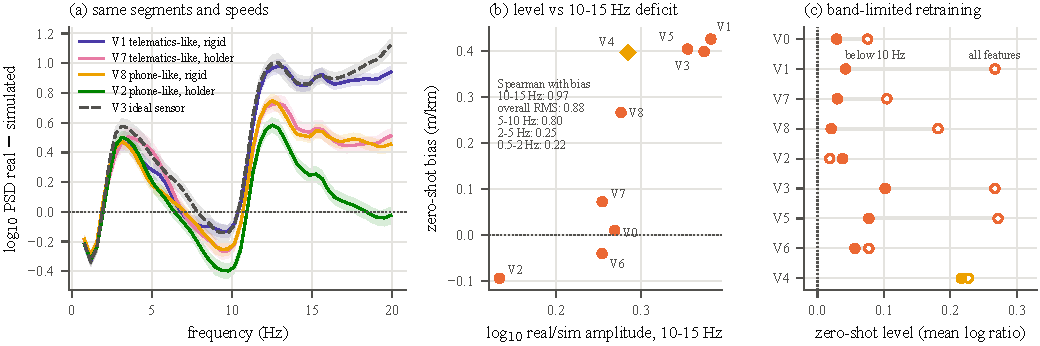
\includegraphics[width=\textwidth]{v3_spectra.pdf}
\caption{(a) Mean difference of log$_{10}$ power spectral density, real minus simulated, on the same segments in the same 10\,km/h speed bands (re-simulated passes of four sensor variants and the ideal sensor; bands: 95\,\% intervals from a 1\,km-block bootstrap). (b) Zero-shot bias of the nine measured-profile variants against the real/simulated amplitude ratio of the 10--15\,Hz band (log$_{10}$; V4: one vehicle), with the Spearman correlation of the bias with the ratio of every band. (c) Mean zero-shot level of each variant with all 13 features and with the five features without content above 10\,Hz.}
\label{fig:spectra}
\end{figure*}

\subsection{Where the simulated vibration differs}
\label{sec:res_mech}

On the same segments and speed bands, the real car's vibration differs from all simulated variants in the same way below 10\,Hz and differently above (Fig.~\ref{fig:spectra}a, Table~\ref{S-tab:s_spectra}): all variants lack energy at 2--5\,Hz (real/simulated power \spVoneMidPow--\spVfiveMidPow) and match it at 5--10\,Hz, whereas at 10--15\,Hz the real car has \spVthreeHighPow{} and \spVoneHighPow{} times the power of the ideal and the rigid telematics-like sensor but only \spVtwoHighPow{} times that of the phone-like sensor with holder resonance.
Across the nine variants the zero-shot bias orders most closely like the amplitude deficit at 10--15\,Hz (Spearman \baSpHighBias), but also like those at 5--10\,Hz (\baSpMidHighBias) and of the overall RMS (\baSpRmsBias), and hardly like those at 0.5--2 and 2--5\,Hz (\baSpLowBias{} and \baSpMidBias; Fig.~\ref{fig:spectra}b, Table~\ref{S-tab:s_band_assoc}); a linear fit explains about as much of the bias with the overall RMS ratio as with the 10--15\,Hz ratio ($R^2$ \baRtwoRmsBias{} and \baRtwoHighBias).
These associations were found after the fact on variants that are not independent, and V4 departs from them: its 10--15\,Hz ratio is close to V0's (\vpVfourRatioHigh{} vs \vpVzeroRatioHigh), its bias is not.
The deficit is larger on motorway than on urban segments for \bgcMotorwayLarger{} of \bgcNvar{} variants (Table~\ref{S-tab:s_gap}), as is the level error.

To test which inputs carry the differences between the sensor variants, we retrained the zero-shot LightGBM of every variant on the \blNfeatLow{} of 13 features that contain no vibration above 10\,Hz (speed, speed variation and the 0.5--2, 2--5 and 5--10\,Hz bands).
Over the eight sensor variants (all but V4), the spread of the mean log level fell from \blFullSpreadLvl{} to \blLowSpreadLvl{} (\blRatioLvl\,\%; urban level \blRatioLvlUrban\,\%, motorway level \blRatioLvlMotorway\,\%) and that of the pooled bias from \blFullSpreadBias{} to \blLowSpreadBias\,m/km, whereas dropping only the 10--15\,Hz band changed every spread by at most \blNoHighMaxChange\,\% (Fig.~\ref{fig:spectra}c, Table~\ref{S-tab:s_band_limited}): the variants differ through all features that carry vibration above 10\,Hz, not through the 10--15\,Hz band alone.
The low-band estimator is not more accurate: for every sensor variant it under-predicts urban and over-predicts motorway segments (log level \blLowLvlUrbanMin{} to \blLowLvlUrbanMax{} and \blLowLvlMotorwayMin{} to \blLowLvlMotorwayMax), and after a 5\,km level offset the pooled MAE of V0--V8 is \blLowCalMin--\blLowCalMax\,m/km instead of \blFullCalMin--\blFullCalMax.
V4 stays outside the range of the sensor variants (mean log level \blLowVfourLvl{} against \blLowLvlMin{} to \blLowLvlMax), so the vehicle population sets part of the level independently of the vibration above 10\,Hz.
The test intervenes on the estimator's inputs, not on the car: it shows where the variant differences enter the estimator, not which physical mechanism produces the real car's extra vibration.

The real car's empirical transmissibility peaks at \invPeakHz\,Hz (Fig.~\ref{S-fig:s_acf}b), and passes logged at 333\,Hz contain more, not less, 10--15\,Hz power than passes logged at 52.6\,Hz on the same cells (52.6 minus 333\,Hz: \spAliasHigh{} in log$_{10}$, confounded with the device), so the excess is not an aliasing artefact.
Its physical source is not identified: the telematics unit is fixed to the frame in the middle console close to the front axle~\cite{skar2023lira}, and the linear half-car omits local modes of the console and its mount, nonlinearity and friction in tyres and suspension, vibration of the electric drivetrain, and roll and body flexibility.
A second mismatch is common to all variants: on a fixed road the real car's vibration RMS rises with speed with elasticity \ssRealUrban{} [\ssRealUrbanLo, \ssRealUrbanHi] on urban and \ssRealMotorway{} [\ssRealMotorwayLo, \ssRealMotorwayHi] on motorway segments, the simulated vibration over the same segments at the same speeds with \ssSimUrbanMin--\ssSimUrbanMax{} and \ssSimMotorwayMin--\ssSimMotorwayMax{} (Table~\ref{S-tab:s_gap}); as this mismatch is similar for all variants, it does not explain their different levels.

\subsection{How much paired real data is needed}
\label{sec:res_value}

Fig.~\ref{fig:value} and Table~\ref{tab:value} compare simulation with paired real drives on the same 20 draws of $k$\,km of training-route road (every variant: Tables~\ref{S-tab:s_value_variants} and~\ref{S-tab:s_value_more}).
Of the two real-only comparators, the vibration index suits very small samples better (pooled MAE \vbRealIdxOne{} vs \vbRealOnlyOne\,m/km for LightGBM at 1\,km).
Ranges over draws reflect which $k$\,km are drawn; intervals over the test routes are in Table~\ref{S-tab:s_calib_unc}.

\begin{figure*}[t]
\centering
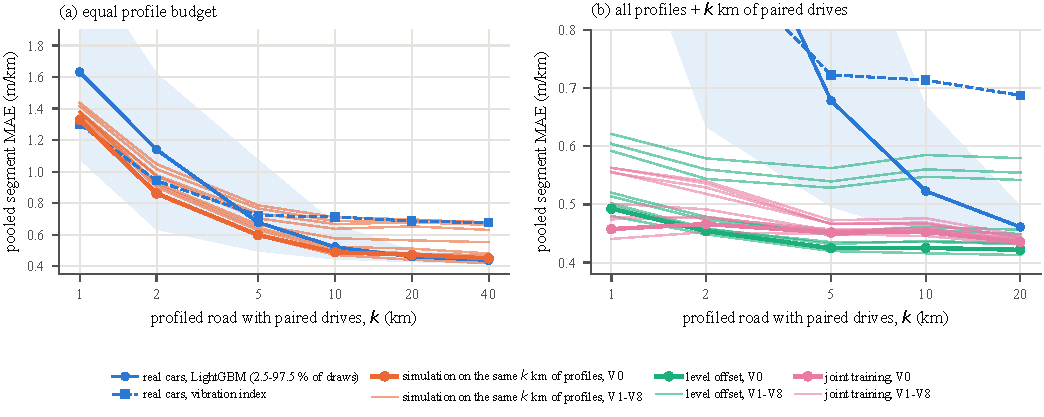
\includegraphics[width=\textwidth]{v3_value.pdf}
\caption{Simulation against paired real drives on the same 20 draws of $k$\,km of training-route road (pooled segment MAE on the held-out routes, means over draws). (a) Equal profile budget: LightGBM on simulated passes over the profiles of the same $k$\,km. (b) Simulation over all training-route profiles combined with the paired passes; real-only values at 1 and 2\,km lie above the axis (LightGBM \vbRealOnlyOne{} and \vbRealOnlyTwo, index \vbRealIdxOne{} and \vbRealIdxTwo\,m/km).}
\label{fig:value}
\end{figure*}

% AUTO-GENERATED by research_rescue/make_tables_v3.py from results/v2 and results/v3 - do not edit by hand.
\begin{table*}[t]
\centering
\caption{Simulation and paired real drives on the same 20 draws of $k$\,km of training-route road (passes: mean number of segment-passes). Pooled MAE (brackets: 2.5--97.5\,\% of draws) and within-route MAE, in m/km. Real-only: LightGBM or the three-parameter vibration index on the paired passes. Equal profile budget: LightGBM on V0 simulated passes over the profiles of the same $k$\,km (difference to real-only LightGBM; draws in which simulation was better). All profiles: simulation over all training-route profiles combined with the paired passes; ranges over V0--V8 of the means, and of the number of draws in which joint training beat real-only LightGBM.}
\label{tab:value}
\setlength{\tabcolsep}{2.6pt}
\scriptsize
\begin{tabular}{@{}rrcccccccccc@{}}
\toprule
& & \multicolumn{3}{c}{Real-only} & \multicolumn{2}{c}{Equal profile budget (V0)} & \multicolumn{2}{c}{All profiles + level offset} & \multicolumn{3}{c}{All profiles + joint training} \\ \cmidrule(lr){3-5}\cmidrule(lr){6-7}\cmidrule(lr){8-9}\cmidrule(lr){10-12}
$k$ & passes & LightGBM pooled & within & index & pooled & $-$ real (better) & pooled & within & pooled & within & better \\
\midrule
1 & 92 & 1.63 [1.08, 2.36] & 1.572 & 1.30 & 1.33 & $-$0.30 (20) & 0.48--0.62 & 0.450--0.576 & 0.44--0.56 & 0.415--0.543 & 20 \\
2 & 184 & 1.14 [0.63, 1.62] & 1.105 & 0.94 & 0.86 & $-$0.28 (20) & 0.45--0.58 & 0.421--0.539 & 0.45--0.54 & 0.426--0.519 & 20 \\
5 & 475 & 0.68 [0.50, 1.07] & 0.629 & 0.72 & 0.60 & $-$0.08 (16) & 0.42--0.56 & 0.395--0.519 & 0.45--0.47 & 0.422--0.445 & 20 \\
10 & 947 & 0.52 [0.45, 0.67] & 0.487 & 0.71 & 0.49 & $-$0.03 (15) & 0.42--0.58 & 0.391--0.537 & 0.45--0.48 & 0.418--0.445 & 18--20 \\
20 & 1,905 & 0.46 [0.43, 0.50] & 0.433 & 0.69 & 0.47 & +0.01 (9) & 0.41--0.58 & 0.388--0.532 & 0.43--0.45 & 0.405--0.419 & 16--20 \\
40 & 3,777 & 0.44 [0.42, 0.47] & 0.412 & 0.68 & 0.45 & +0.01 (3) & -- & -- & -- & -- & -- \\
\midrule
all & & 0.42 & 0.395 & -- & 0.44 (zero-shot) & -- & -- & -- & -- & -- & -- \\
\bottomrule
\end{tabular}
\end{table*}


\emph{Equal profile budget} (Fig.~\ref{fig:value}a).
Simulated drives over the profiles of the $k$\,km are no general substitute for the real drives over them: with 1--2\,km, simulated LightGBM beats real-trained LightGBM for every variant but not the real-trained index (better in \pcSameWinsIdxOneMin--\pcSameWinsIdxOneMax{} of 20 draws at 1\,km), and from 5\,km on the answer depends on the variant (at 20\,km, \pcSameDiffTwentyMin{} to \pcSameDiffTwentyMax\,m/km against real-only LightGBM, largest for V1, V3 and V5, the variants with the largest 10--15\,Hz deficit); a level offset from the same $k$\,km closes the gap of V4 (\pcSameCalVfourDiffTwenty\,m/km) but not theirs.

\emph{All profiles plus paired drives} (Fig.~\ref{fig:value}b).
Trained on simulated drives over all profiled training roads and combined with 5\,km of paired drives, every variant beats training on those drives alone (pooled MAE \vbRealOnlyFive\,m/km), whether the paired drives set a level offset (\pcCalMaeFiveMin--\pcCalMaeFiveMax\,m/km, better in \pcCalWinsFiveMin--\pcCalWinsFiveMax{} of 20 draws) or enter joint training with the simulated units (\poMaeFiveMin--\poMaeFiveMax\,m/km, better in \poWinsFiveRange{} of 20 draws).
The test-route intervals exclude zero for every variant and both combinations (differences \cuCalFiveDiffMin{} to \cuCalFiveDiffMax{} and \cuPoolFiveDiffMin{} to \cuPoolFiveDiffMax\,m/km), and within-route MAEs agree (Table~\ref{tab:value}).
With more paired data the two combinations diverge.
Real-only LightGBM overtakes the level offset of V1, V3 and V5, which is better in only \pcCalHiDefWinsTenMin--\pcCalHiDefWinsTenMax{} of 20 draws at 10\,km and in none at 20\,km (test-route intervals above zero; differences \cuCalVoneTwenty{} to \cuCalVfiveTwenty\,m/km), whereas joint training stays better than real-only LightGBM for every variant up to 20\,km (\poDiffTwentyMin{} to \poDiffTwentyMax\,m/km at 20\,km, better in \poWinsTwentyRange{} of 20 draws, every test-route interval below zero).
Per held-out route it is better in \poRouteTwentyNeg{} of the \poRouteTwentyCells{} combinations of variant and route at 20\,km; the other \poRouteTwentyPos{} (\poRouteTwentyMwThreePos{} on M3, \poRouteTwentyCphSixPos{} on CPH6) differ by at most \poRouteTwentyDiffMax\,m/km.
With joint training the variant matters little from 5\,km on (the nine variants span \poMaeSpreadFive\,m/km at 5 and \poMaeSpreadTwenty\,m/km at 20\,km, against \poCalSpreadFive{} and \poCalSpreadTwenty\,m/km with a level offset), but it still matters at 1\,km (\poMaeOneMin--\poMaeOneMax\,m/km).

Which combination is better depends on the kind of level error.
A level offset removes a common level and leaves the difference between the motorway and urban levels, which ranges from \ldSpreadMin{} to \ldSpreadMax{} over V0--V8 (Table~\ref{tab:variants}) and orders their MAE after the offset (Spearman \ldSpreadCalRho).
At 5\,km, joint training minus level offset is \poHiDefDiffCalFiveMin{} to \poHiDefDiffCalFiveMax\,m/km for V1, V3 and V5, whose class difference is largest (\ldHiDefSpreadMin--\ldHiDefSpreadMax), and \poLoDefDiffCalFiveMin{} to \poLoDefDiffCalFiveMax\,m/km for the other six (\ldLoDefSpreadMin--\ldLoDefSpreadMax).
An affine map fitted to the paired passes was less accurate than the better of the two for \poAffWorseFive{} of 9 variants at 5\,km and \poAffWorseTwenty{} of 9 at 20\,km (Table~\ref{S-tab:s_value_more}).

LiRA-CD drives each segment about ten times, but with simulation far fewer passes suffice: keeping at most one pass per segment of the 5\,km (\pdUnitsOne{} instead of \kdUnitsFive{} segment-passes on average) hardly changed the combinations with simulation (level offset \pdCalOneMin--\pdCalOneMax\,m/km, joint training \pdPoolOneMin--\pdPoolOneMax), which stayed better than real-only LightGBM on the same passes \pdOneAllDraws{} for every variant, whereas real-only LightGBM degraded from \vbRealOnlyFive{} to \pdRealOne\,m/km (Table~\ref{S-tab:s_pass_density}).
The simulation also contributes more than a speed exponent and a slope: a vibration index $\log\mathrm{IRI}=c+b\log(\mathrm{RMS}/v^{\alpha})$ with the car's own speed exponent ($\alpha=$\,\nsAlphaCarMin--\nsAlphaCarMax, estimated without labels within segments of the training routes) and an affine fit to the same paired passes reaches \nsCarAffineFive\,m/km at 5\,km and \nsCarAffineTwenty\,m/km at 20\,km.

\subsection{Speed dependence on a fixed road}
\label{sec:res_speed}

On a fixed road (median within-segment SD of log speed \elSdLogv; Fig.~\ref{S-fig:speed}, Table~\ref{S-tab:s_speed}; 1\,km-block intervals for single elasticities), the real car's vibration RMS rises by \elRawPooledPct\,\% between 40 and 100\,km/h (elasticity \elRawPooled{} [\elRawPooledLo, \elRawPooledHi]).
The estimators trained on real cars over-correct for it: LightGBM's estimate falls by \elRealGbmPooledPct\,\% over the same range (\elRealGbmPooled{} [\elRealGbmPooledLo, \elRealGbmPooledHi]), also without speed inputs (\elRealGbmNoSpeedPooled), the MLP and CNN behave alike (\elRealMlpPooled{} and \elRealCnnPooled), and the vibration index over-corrects most (\elRealIdxPooled).
Simulation-trained LightGBM V0 changes by \elSimGbmPooledPct\,\% (\elSimGbmPooled{} [\elSimGbmPooledLo, \elSimGbmPooledHi]); paired on the same passes, its elasticity exceeds that of the real-trained model by \epVzeroPooled{} [\epVzeroPooledLo, \epVzeroPooledHi] (5\,km blocks), entirely on urban roads (\epVzeroUrban{} [\epVzeroUrbanLo, \epVzeroUrbanHi]; motorways \epVzeroMotorway{} [\epVzeroMotorwayLo, \epVzeroMotorwayHi]).
Across the nine variants the paired difference ranges from \epMeasPooledMin{} to \epMeasPooledMax{} (interval excluding zero for \epMeasPooledExcl{} of 9), and on motorways every estimate falls with speed.
These elasticities change little with telematics-unit fixed effects or with the within-pass speed SD as a covariate (Table~\ref{S-tab:s_speed_rob}), except that slow urban passes are more dynamic (within-segment correlation of log speed and log speed SD \srCorrLsdUrban): with the speed SD as a covariate the real-trained urban elasticity shrinks to \srRealUrbanLsd{} [\srRealUrbanLsdLo, \srRealUrbanLsdHi], while the paired urban difference stays at \srDiffUrbanLsd{} [\srDiffUrbanLsdLo, \srDiffUrbanLsdHi].
The speed coefficient of variation, tied to $1/v$ by construction (correlation \srCorrCvUrban{} with log speed), absorbs most of the speed variation within urban segments and turns that difference negative (\srDiffUrbanCv{} [\srDiffUrbanCvLo, \srDiffUrbanCvHi]), so on urban roads speed and speed variability cannot be fully separated.
The smaller urban over-correction of simulation-trained LightGBM thus holds with the unit and speed-SD controls but not with the speed-CV control, so it is not established; simulation did not make estimates speed-invariant, and given the speed-scaling mismatch of Section~\ref{sec:res_mech} any difference reflects the learned estimators, not a reproduced speed response of the car.
